\documentclass[]{article}
\usepackage{graphicx}
\usepackage{caption}
\usepackage{subcaption}
%opening
\title{ECE 657A Assignment \#2}
\author{Yuzhou Wang (20609396), Laura McCrackin (20262085), \\ and Huang Tianhui (20587328)}


\begin{document}

\maketitle


%%\begin{figure}
%\includegraphics{../images/741741}
%%\end{figure}

\section{Parameter Selection and Classification}

\subsection{Preprocessing}

For the original dataset D, we observed that there are no missing values and that the values for all points are close to the mean, so we simply used Z-score normalization to preprocess the data without any further outlier correction. As directed, we use the first half of data for training, and the second half for testing.

\subsection{K-NN}

To perform 5-fold cross validation, the training data was divided randomly into 5 partitions using the ``crossvalind" function.  Four of these partitions were used for training, with the fifth being using for testing; k-NN was run five times in this manner, so that each of the five training partitions in turn was used as the testing set while the remaining partitions were used as training.  The cross-validation accuracy was then taken to be the average accuracy for each of these five trials.

This cross validation process was performed for each $k$ value, $k$=1,3,5...31.  It should be noted that since the cross validation partitioning is random, the $k$ value producing the highest classification accuracy is not the same every time this experiment is performed.  

%For 5-fold cross validation, we could use the function "crossvalind", and use "fitcknn" to find K-NN neighbours. And for the calculation of accuracy, we could use "predict" function to judge the reality result is how similar with the theoretical result. And instead of the loop, every time we compare the best k, so that we could get the best K. For run time calculate, we could use "tic", "toc" function directly. By spiting data into training data and test data, and judge the result, we could get the truth positive, truth negative, false positive and false negative respectively. For more details, could reference the code.


\begin{figure}[h!]
	\centering
	\begin{subfigure}{.49\textwidth}
		\centering
		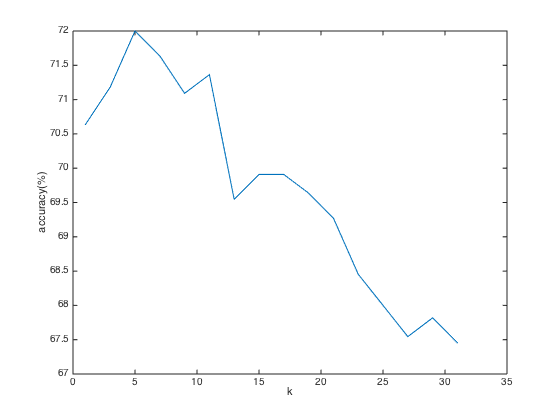
\includegraphics[width=1\linewidth]{../images-update/1-(2)-1.png}
		\caption{best k=5}
%		\label{fig:sub1}
	\end{subfigure}
	\begin{subfigure}{.49\textwidth}
		\centering
		%TODO IS THIS THIE RIGHT PICTURE?! moved from folder 1
		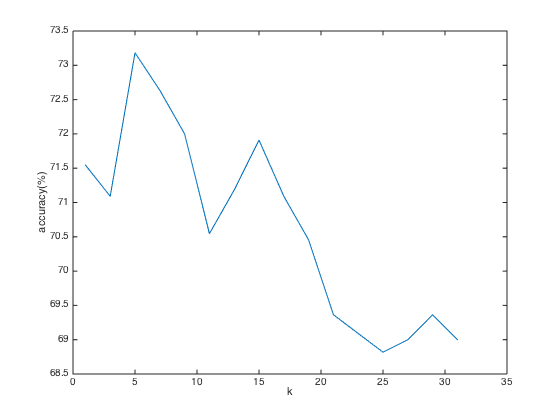
\includegraphics[width=1\linewidth]{../images-update/1-(2)-2.png}
		\caption{best k=5}
		\label{fig:sub1}
	\end{subfigure}
	%\caption{Data histograms before normalization.}
	%\label{fig:hist1}

	\begin{subfigure}{.49\textwidth}
		\centering
		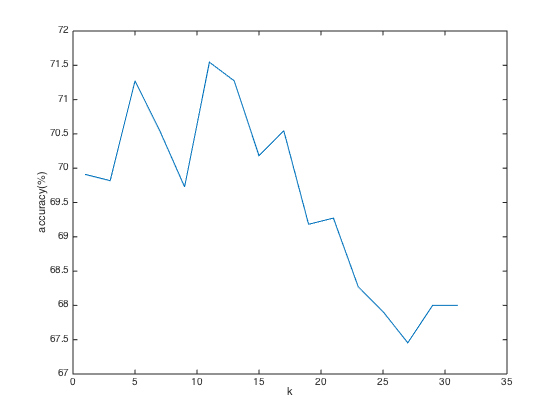
\includegraphics[width=1\linewidth]{../images-update/1-(2)-3.png}
		\caption{best k=12}
		\label{fig:sub1}
	\end{subfigure}
	\begin{subfigure}{.49\textwidth}
		\centering
		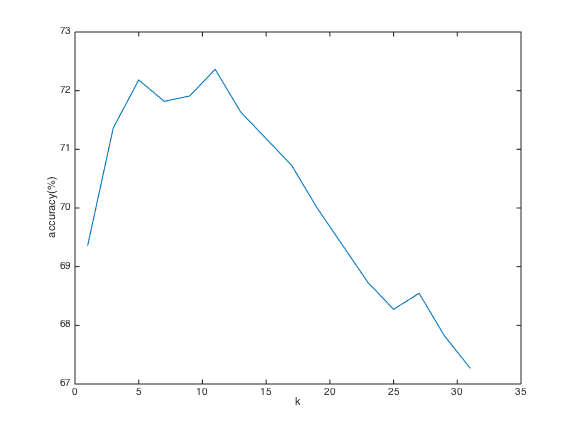
\includegraphics[width=1\linewidth]{../images-update/1-(2)-4.png}
		\caption{best k=12}
		\label{fig:sub1}
	\end{subfigure}		
		\caption{Different cross-validation experiments and their results}
	\label{fig:knn}
\end{figure}

In Figure \ref{fig:knn}, the classification accuracy for k-NN can be observed for four sample runs.  As can be seen, each time the value of best $k$ changes; it is consistently between 5-12 with an accuracy of between 71\% and 73\%.

%We could also notice that when k is smaller than the range of best k, the accuracy increased and later larger the largest best k, it decreased. I think maybe it is the reason that less than k points is to small to be a class, in other words, less points can not represent a class, but if K is too large, then it means that some other class' points maybe be included, which leads to a lower accuracy. Lastly, since we randomly choose the dataset and split them so that there could be some flexible results also.
%And what is more, we should also notice about the accuracy about the dataset itself, maybe there are some outliers. And what is more, since it is DNA sequence, it means some cuts may represent nothing, but it still appears at the dataset with a label. Above all, the result we get maybe not the exactly right answer.




\subsection{SVM with RBF Kernel}

Next, we perform a grid search to determine the best combination of $c$ and $gamma$ values for classifying our dataset using an SVM with a radial basis function (RBF) kernel.  That is, we perform 5-fold cross-validation for each combination of candidate $c$ and $gamma$ values, for $c$ = 0.1, 0.5, 1, 2, 5,
10, 20, 50 and $gamma$ = 0.01, 0.05, 0.1, 0.5, 1, 2,
5, 10.

The resulting ROC curve may be seen in Figure \ref{fig:roc}.  The optimal combination of parameters can be seen as the innermost point of the curve.

%According to the best c and gamma, we could trace the ROC plot.C is the cost of classification as correctly stated, a large C gives you low bias and high variance. Low bias because you penalize the cost of misclassification a lot. A small C gives you higher bias and lower variance. Gamma is the parameter of a Gaussian Kernel (to handle non-linear classification). For non-linear classification, gamma controls the shape of the "peaks" where you raise the points. A small gamma gives you a pointed bump in the higher dimensions, a large gamma gives you a softer, broader bump.So a small gamma will give you low bias and high variance while a large gamma will give you higher bias and low variance. Theoretically with the increasing of gamma(kennel width), the accuracy decrease, because if the gamma is small enough(nearly 0), then it means that data point is not influenced or correlated with other data points. Small kernel width may cause over-fitting, and large one under-fitting. The so-called optimal kernel width is merely selected based on the tradeoff between under-fitting loss and over-fitting loss. 

\begin{figure}[h!]
	\centering
		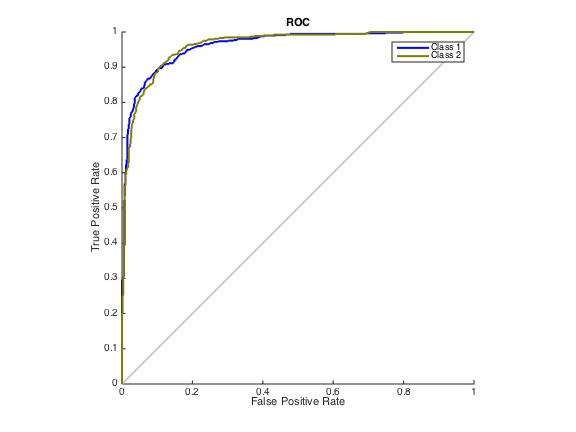
\includegraphics[width=.8\linewidth]{../images-update/1-(3)-2.png}
		\caption{ROC}
		\label{fig:roc}	 
\end{figure}


\subsection{Comparison of Methods}
We then perform a comparison of k-NN, SVM using an RBF kernel, a Naive Bayes classifier, a Decision Tree (using the ``fitctree" function), and a Neural Network (using ``patternnet").  The SVM and k-NN were run using the aforementioned ideal values, while the remaining methods were used with default parameters.  All experiments were repeated 20 times, with the classification accuracy averaged for all trials.

%Since we need to calculate the data result for 20 times, so define different matrix result and all the initial values are all 0. For Naive Bayes classifier function could use "fitNaiveBayes" function directly, the training process or calculate true positive are all similar to the above method. And for decision tree classifier could use function "fitctree" and method also similar to the above. For neural network, we could first create a neutal network by the function of patternnet and hidden layer by default is 10. For training method, we could use "train" function, and label different networks according to the test result, by setting and labelling class by hand, we could better compare with test set.

From the accuracy table above, we can see that the Decision Tree provides the highest accuracy, precision, recall and F-measure values, but also requires the most time to run. The worst performance is achieved using k-NN.

%For neural network, we could see the result in picture performance".  Generally, the error reduces after more epochs of training, but might start to increase on the validation data set as the network starts overfitting the training data. In the default setup, the training stops after six consecutive increases in validation error, and the best performance is taken from the epoch with the lowest validation error. Next we could see figure "neural-confusion". Since result – outputs = targets. The R value is an indication of the relationship between the outputs and targets. If R = 1, this indicates that there is an exact linear relationship between outputs and targets. If R is close to zero, then there is no linear relationship between outputs and targets. We could see the result for test, validation and train group, the result is around 50\%, so it is not really good or not really bad. For ROC graph, we could see the figure "neural-receiver", for training, validation and test ROC, they all have better performance since it is above 0.5. For neural-gradient
%figure, we could see that the trend of gradient is nearly stable, since it represents the slope of the tangent of the graph of the function. It means that there is no significant increasing or decreasing(this picture not sure). From the figure "netural-error", we could see that around the 0 errors, it has the best result.(this picture also not sure)
%For this example, the training data indicates a good fit. The validation and test results also show R values that greater than 0.9.

\begin{figure}[h]
	\centering
	\begin{subfigure}{.49\textwidth}
		\centering
		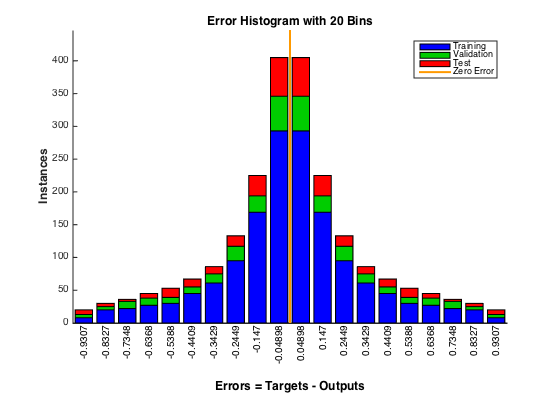
\includegraphics[width=1\linewidth]{../images-update/1-(4)-netural-error.png}
		\caption{netural-error}
		\label{fig:sub1}
	\end{subfigure}
	\begin{subfigure}{.49\textwidth}
		\centering
		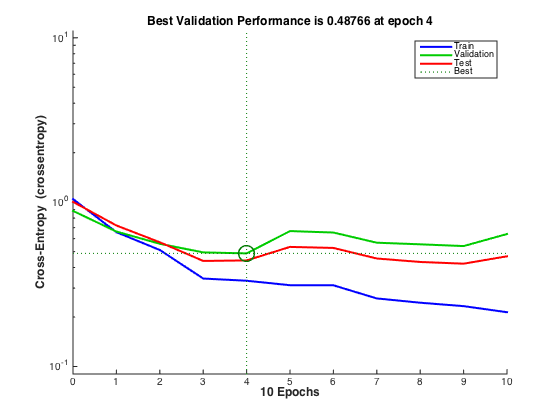
\includegraphics[width=1\linewidth]{../images-update/1-(4)-neural-perfomance.png}
		\caption{perfomance}
		\label{fig:sub1}
	\end{subfigure}
	%\caption{Data histograms before normalization.}
	%\label{fig:hist1}
	
	\begin{subfigure}{.49\textwidth}
		\centering
		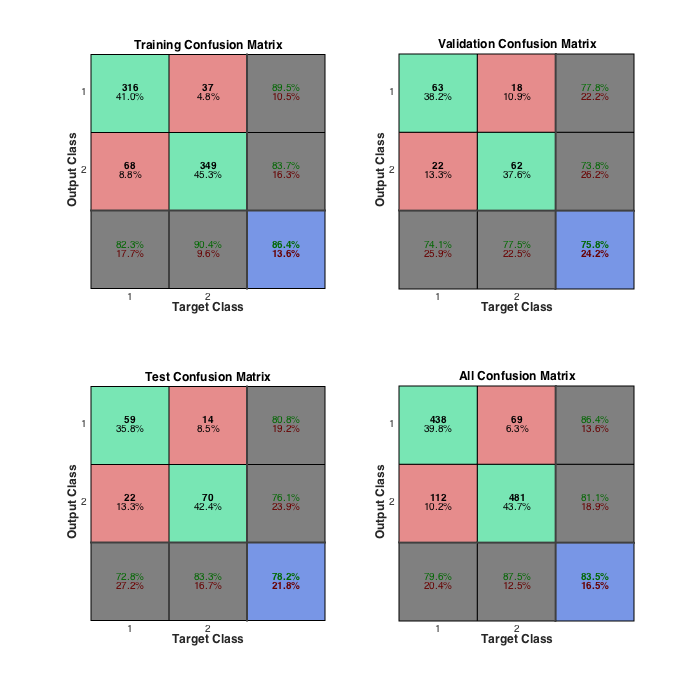
\includegraphics[width=1\linewidth]{../images-update/1-(4)-neural_confusion.png}
		\caption{neural-confusion}
		\label{fig:sub1}
	\end{subfigure}	
	\begin{subfigure}{.49\textwidth}
		\centering
		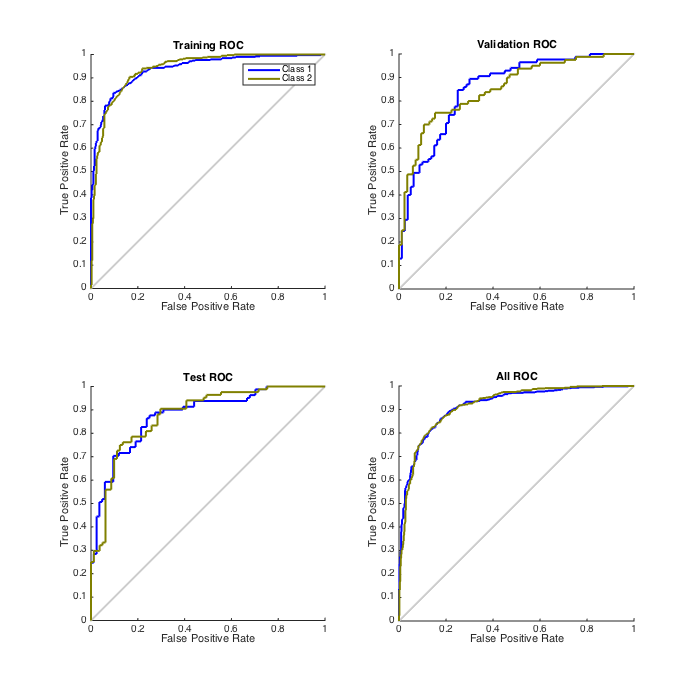
\includegraphics[width=1\linewidth]{../images-update/1-(4)-neural_receiver.png}
		\caption{neural-receiver}
		\label{fig:sub1}
	\end{subfigure}
	
	\begin{subfigure}{.5\textwidth}
		\centering
		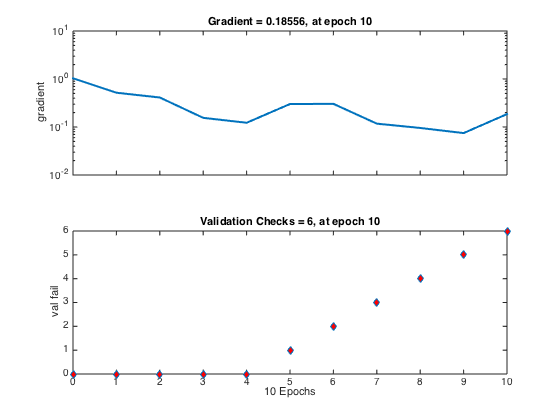
\includegraphics[width=1\linewidth]{../images-update/1-(4)-neural_gradient.png}
		\caption{neural-gradient}
		\label{fig:sub1}
	\end{subfigure}
	
	
	\end{figure}
	
	
\begin{tabular}
	{l*{6}{c}r}   	& K-NN  & RBF SVM & Naive Bayes & Decision Tree & Neural Net \\ \hline
	Accuracy & 74.4182 & 89.1864 & 86.4864 & 92.9818 & 82.5773 \\ 
	std accuracy & 1.2322 & 0.7382 & 0.6734 & 0.9843 & 1.7322 \\ \hline
	Precision & 0.9104 & 0.9113 & 0.8603 &0.9391 & 0.8461\\
	std Precision & 0.028 & 0.0131 & 0.0101 & 0.0146 & 0.0240\\ \hline
	Recall & 0.5415 & 0.8764 & 0.8810 & 0.9250 & 0.8089\\
	std recall & 0.0293 & 0.0097 & 0.0104 & 0.0126 & 0.0330\\ \hline
	F-measure & 0.6782 & 0.8934 & 0.8705 & 0.9319 & 0.8265 \\
	std F-measure & 0.0195 & 0.0070 & 0.0060 & 0.0093 & 0.0186 \\ \hline
	Training time (s/sample) &  0.0081 & 0.1028 & 0.0093 & 0.00518 & 0.2698 \\
	Class. time (s/sample) & 0.008 & 0.0690 & 0.0026 & 0.0104 & 0.0082 \\ \hline
\end{tabular}

\subsection{Strengths and Weaknesses}
For test accuracy, it could be reflected by accuracy, precision and f-measure. At the same time we could also combine the std to see the stable result.Precision is how useful the search results are, and recall is how complete the results are.high precision means that an algorithm returned substantially more relevant results than irrelevant, while high recall means that an algorithm returned most of the relevant results.Recall is defined as the number of relevant documents retrieved by a search divided by the total number of existing relevant documents, while precision is defined as the number of relevant documents retrieved by a search divided by the total number of documents retrieved by that search. For f-measure, it considers both the precision p and the recall r of the test to compute the score: p is the number of correct positive results divided by the number of all positive results, and r is the number of correct positive results divided by the number of positive results that should have been returned. The F1 score can be interpreted as a weighted average of the precision and recall, where an F1 score reaches its best value at 1 and worst at 0.


From the above table, we could get the conclusion that Decision tree method could get the highest accuracy. The std accuracy is also has a relatively low level, so it means the average result is relatively stable. For the precision and std precision, all of the methods have a good performance, but maybe the best one is still the decision tree method.For recall and std recall, we could also get the conclusion that decision tree method and neural network have better performance, which means that the true positive divided by the correct answer for both true positive and false negative is high. Similarly, the decision tree method also have the good performance for f-measure and std-measure.

For classification time in K-NN, it should compare all test samples with test samples. For time percepective, naive bayes has the best performance and also have the lowest time value. 

So we could choose decision tree method for both time saving and higher accuracy. 

%K-NN: Training a k-NN classifier simply consists of determining k and preprocessing documents. In fact, if we preselect a value for k and do not preprocess, then kNN requires no training at all. It means that for K-NN, there is no training process and for the classification process, compare the test sample with all of the samples, the time measure has been divided by all of samples.But the disadvantage of K-NN is that irrelevant dimensions could have bad influence a lot.

%For SVM: For linear SVMs, at training time you must estimate the vector w and bias b by solving a quadratic problem, and at test time prediction is linear in the number of features and constant in the size of the training data. For kernel SVMs, at training time you must select the support vectors and at test time your complexity is linear on the number of the support vectors (which can be lower bounded by training set size * training set error rate) and linear on the number of features (since most kernels only compute a dos product; this will vary for graph kernels, string kernels, etc).So from the above the SVM maybe the time consuming most.SVMs contain an underlying optimization step that is solved heuristically, so for any actual algorithm that purports to solve SVMs, the answer is undefined. A number like O(n*n*n)is generally bandied around for implementations like libsvm, which means something like time/iteration * number of iterations (where numbr of  iterations is assumed to be constant)



%Naïve Bayes Classifier: As we could conclude from the table that it is the most efficient method, linearly proportional to the time needed to just read in all the data.

%Decision Trees: Decision trees are easy to use compared to other decision-making models, but preparing decision trees, especially large ones with many branches, are complex and time-consuming affairs.Computing probabilities of different possible branches, determining the best split of each node, and selecting optimal combining weights to prune algorithms contained in the decision tree are complicated tasks that require much expertise and experience.Decision trees moreover, examine only a single field at a time, leading to rectangular classification boxes. This may not correspond well with the actual distribution of records in the decision space.In reality, the complexity in creating large decision trees mandates people involved in preparing decision trees having advanced knowledge in quantitative and statistical analysis. This raises the possibility of having to train people to complete a complex decision tree analysis. The costs involved in such training makes decision tree analysis an expensive option, and remains a major reason why many companies do not adopt this model despite its many advantages. But the advantage of this method is it provide easy way to view illustrations.


%Neural Networks: Since for each layer it could be lots of combination, and the number of layers are not a certain number for different situation, so this method could be time consuming.(not sure about this part analyse)



\section{Clustering Analysis}
\subsection{Hierarchical Clustering Using Agglomerative Algorithms}
\subsubsection{Comparison of Linkage Methods}
We use the Matlab library function `clusterdata' to perform clustering using single, complete, and ward linkage methods, respectively.

To find the separation index, we calculate the centre of each cluster and calculate the square of the distance from each point to the centre point. This result is then divided by the total number of rows multiplied by the maximum distance for each cluster. For rand-index, it should be calculated by $(a+d)/M$, where $a$ is the number of True Positives and $d$ is the number of False Negatives, with $M$ being the total number of possible point comparisons. For F-measure, we first calculate the precision and recall, and then use the function:   
$F(i,j) = 2*precision(i,j)* recall(i,j)/(precision(i,j)+recall(i,j)).$


According to the definition, the separation index is highly dependant on the clustering results. Smaller separation index means that every point in the cluster is close and as a result there could be more groups.
The result of rand-index and f-measure could have the similar trend for representing accuracy of the same cluster group, which is corresponding different with separation-index. It means that if there is a higher accuracy for cluster, the rand-index and f-measure could correspondingly higher, but it means larger size of cluster, as a result separation-index could be lower.



There are two ways to calculate the separation index; one is for the maximum distance and another is for minimum distance. Below the first table shows the result for the maximum distance.
For maximum distance method:

%For linkage method=single\\
%Separation-Index=1.7540 \\
%Rand-Index=0.1097\\
%F-measure= 0.0962\\

%For linkage method=complete\\
%Separation-Index=0.6151 \\
%Rand-Index=0.8184 \\
%F-measure=0.2168\\

%For linkage method=ward\\
%Separation-Index=0.4937 \\
%Rand-Index=0.8772 \\
%F-measure= 0.2801 \\


\begin{tabular}
	{l*{3}{c}r}   	& Single  & Complete & Ward \\ \hline
	Separation-Index& 1.7540 & 0.6151 & 0.4937  \\ 
	Rand-Index & 0.1097 & 0.8184 & 0.8772 \\
	F-measure & 0.0962 & 0.2168 & 0.2801 \\
	

\end{tabular}



When we choose the maximum method, the smaller the value it is, the closer for the points are within a class and the greater the separation from other classes. A smaller SI value is therefore ideal. The opposite is true for rand-index and f-measure. So, the ward algorithm has the best result, having the smallest separation-index and the largest rand-index and f-measure values. 

\subsubsection{Optimal Number of Clusters}

After we run the `ward' algorithm for a variety of cluster numbers, we found the optimal value to be 15.

\subsection{Clustering Using K-Means}

The result of using k-means can be seen in Figure \ref{fig:kmeans}. We could see that both rand-index increase a lot with the increasing number of cluster, and f-measure increase a lot at the beginning and later a little bit decrease, but separation-index decrease.

The reason why rand-index increase is because of the calculating function with the increasing number of cluster, it is closer to the right cluster way, but for the value of M it did not change, so it has an increasing trend. Similarly, f-measure also increase, for increasing number of clusters, it could reflect better accuracy. And for the separation-index, with the increasing number of cluster the value of SI should also decrease for more densy in the same group and more distance for different class. Above all, all the three methods shows that the increasing number of clusters leading to a better result.

Combined with three methods, the best cluster number is 8, without too high separation-index or too low rand-index and f-measure.


\begin{figure}[h]
	\centering
	\begin{subfigure}{.9\textwidth}
		\centering
		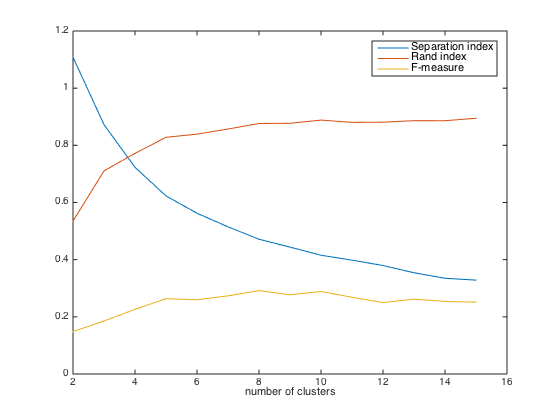
\includegraphics[width=1\linewidth]{../images-update/2-(2)-3.png}
		\caption{K-means algorithm}
		\label{fig:kmeans}
	\end{subfigure}
	
	
	
\end{figure}



\subsection{Fuzzy C-Means}


\subsubsection{Cluster Membership}

For the fuzzy c-means methods, we could use `fcm' function directly, and label the result is same with digit `1' or `3', so that we could get the graphs in Figure \ref{fig:1vs3}.

\begin{figure}[h]
	\centering
	\begin{subfigure}{.49\textwidth}
		\centering
		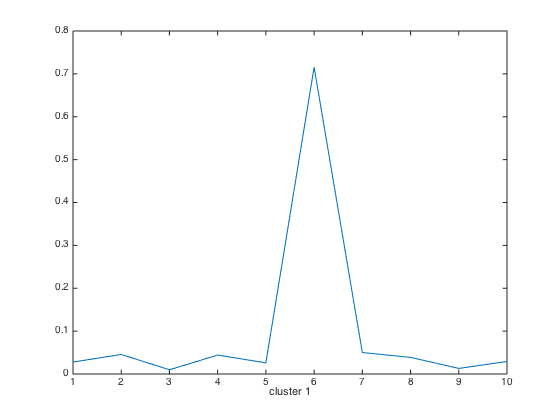
\includegraphics[width=1\linewidth]{../images-update/2-(3)-(a)-2.png}
		\caption{Digit 1}
		\label{fig:sub1}
	\end{subfigure}
	\begin{subfigure}{.49\textwidth}
		\centering
		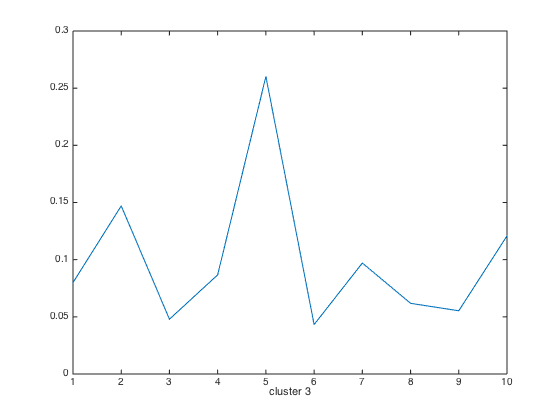
\includegraphics[width=1\linewidth]{../images-update/2-(3)-a-1.png}
		\caption{Digit 3}
		\label{fig:sub1}
	\end{subfigure}
	\caption{Points from digits 1 and 3 in each cluster (out of 1.0)}
	\label{fig:1vs3}
\end{figure}
From the graph, we could see that, for digit 1, it mainly in cluster 5 to 7, without too much overlapping with other groups. However, the result of digit 3 could be checked in different clusters, which means that there are more overlaps in cluster 3 but less in cluster 1. For the reason why there is less overlapping for digit 1 maybe for the hand writing dataset, the digit `1' is hard to make confusing with other digits unlike digit `3', which is similar to the digit 8, for example.
 
\subsubsection{Hard Clustering}

In fuzzy clustering (also referred to as soft clustering), data elements can belong to more than one cluster, and associated with each element is a set of membership levels. But in hard clustering, data is divided into distinct clusters, where each data element belongs to exactly one cluster. Hard clustering can perhaps be considered a less flexible method, where the subtleties of classification uncertainty reflected in fuzzy clustering are no longer retained.

For Fuzzy c-means\\
Separation-index=0.4454\\
Rand-Index=0.8905\\
F-measure=0.2844\\

For linkage method=single\\
Separation-Index=1.7540 \\
Rand-Index=0.1097\\
F-measure= 0.0962\\
For linkage method=complete\\
Separation-Index=0.6151 \\
Rand-Index=0.8184 \\
F-measure=0.2168\\
For linkage method=ward\\
Separation-Index=0.4937 \\
Rand-Index=0.8772 \\
F-measure= 0.2801 \\

As can be seen above, fuzzy-c means has better performance than the other three methods.



\end{document}